\section{Model, task, and what counts as failure}
\label{sec:model}

\paragraph{Serial spectral--spatial model.}
An input is an image whose pixel $p$ carries a spectrum $x_p\in\R^S$ and a
label $y_p\in\{-1,+1\}$. A spectral encoder $f_\thetap:\R^S\to\R^K$ acts on
each pixel separately, and a spatial model $g_\phip$ of width $M$ reads the
encoded neighbourhood of $p$ to produce a logit $F_p$. The encoder is
linear, $f_\thetap(x)=Wx$ with $W\in\R^{K\times S}$, in the theorem and in
the experiments; the spatial model is a replicated readout in the theorem
and a ReLU convolutional head in the experiments. Training minimizes the
mean margin loss $\loss=\frac1N\sum_p\log(1+e^{-y_pF_p})$ by gradient flow
or plain gradient descent with a base rate $\eta$; the baseline uses that
one rate for every parameter, and the interventions multiply the rate of
a named block by a stated factor, so that every difference in training
speed between the modules is either a property of the model or an
explicit, declared multiplier.

\paragraph{Two cues.}
The training distribution carries the label in two places. The
\emph{spectral cue} lies in the pixel's own spectrum along a direction the
encoder must discover: a randomly initialized encoder attenuates it. The
\emph{contextual cue} lies in the neighbourhood along directions of large
amplitude: a randomly initialized encoder passes it, so a trained readout
can use it at once. The two cues are calibrated to matched discriminant
accuracy on calibration data (a matched signal-to-noise construction in
the synthetic case; a training-side estimate on real spectra), so that a
preference for one cue is not simply a preference for the more predictive
one. The theorem allows any $(a_0,v_0)$; the experiments select its
regime of interest, a small initial spectral contribution and an
initially accessible contextual one, and measure that accessibility
asymmetry directly (Section~\ref{sec:synthetic}).

\paragraph{Matched fit, spectral learning, reliance, failure.}
We compare models at their first attainment of a prespecified
training-fit threshold: a common margin in the solvable model and mean
training loss in the experiments. Spectral learning means adaptation of
the designated spectral coefficient in the theorem and increased
independently measured linear accessibility of the centre's spectral cue
in the experiments. We measure contextual reliance by changing the
assigned contextual signal while preserving the target's spectral cue,
label and noise, and recording the resulting change in predictions or
risk. We call that reliance a failure when the shifted risk exceeds that
of a comparator of the same architecture trained with an uninformative
(decorrelated) context to the same fitting threshold. The theorem supplies
an exact reversal failure against a spectral-only model; the noisy
experiments measure the corresponding risk difference against that
trained comparator, without assuming a zero-error reference. Four
measurements are kept distinct throughout: adaptation of the encoder,
linear accessibility of the spectral cue on clean spectral inputs (the
probe), use of context by the original predictor, and performance after
an explicit retraining procedure.

\paragraph{Test conditions.}
Every evaluation family is generated from the same labels and noise in
several ways: \emph{iid} (context agrees with the label as in training),
\emph{reversed} (the assigned context carries the opposite label) and
\emph{context-random} (the assigned context carries an independent label,
so context is present but uninformative). In the synthetic experiment the
intervention changes the contextual feature field at every pixel while the
target's spectral component, label and noise are shared; in the
real-spectrum experiment each centre spectrum is held fixed and only its
neighbours change. Accuracy under reversal measures reliance; accuracy
under context-random measures what the original predictor does from the
spectrum in the presence of context.

\begin{figure}[t]
\centering
\IfFileExists{figures/fig1_model.pdf}{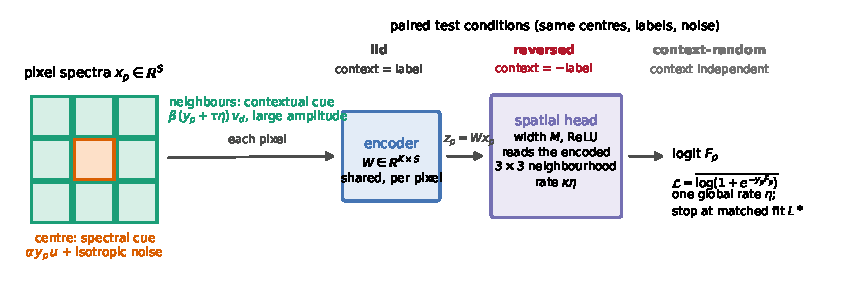
\includegraphics[width=0.92\linewidth]{figures/fig1_model.pdf}}{\fbox{\rule{0pt}{1.6in}\rule{0.97\linewidth}{0pt}}}
\caption{The serial model and the two cues. Each pixel's spectrum passes
through the shared encoder; the spatial model reads the encoded
neighbourhood (a $5\times5$ receptive field from two $3\times3$
convolutions in Experiment 2; one nine-spectrum patch in Experiment 3).
The contextual cue is placed in the eight nearest neighbours along
large-amplitude directions that a random encoder already passes; the
spectral cue sits in the pixel's own spectrum along a direction of small
amplitude and, in the low-accessibility settings, requires encoder
alignment. Evaluation under iid, reversed and context-random contexts
measures reliance and failure.}
\label{fig:model}
\end{figure}
